
\subsection{Multivariate rational approximations}
\label{sec-rapp}

Rational approximations can be seen as natural extensions of the polynomial
approximations used so far in PROFESSOR. Denoting the degrees of the numerator 
and denominator polynomial as $m$ and $n$ respectively, we can formally define
the rational approximation as
\begin{equation}\label{eq:rappdef}
    f^{(m,n)}(p) = \frac{h^{(m)}(p)}{g^{(n)}(p)}.
\end{equation}
Polynomial approximations in this picture are thus simply the class of rational approximations with $n=0$.

\subsection{The algorithm}

For simplicity, we present the algorithm for a one-dimensional parameter space. We are interested in deriving a rational approximation:
\begin{equation}\label{eq:PadeOneD}
  f : \R \to \R, \quad f(p) \simeq \frac{h(p)}{g(p)}
\end{equation}
by fitting the coefficients of $h(p), g(p)$ to data, $(p_l, f(p_l)$. Denoting the polynomials
as
\begin{equation}
  h(p) = a_0 + a_1 p + a_2 p^2 + \ldots + a_m p^m \quad \text{and} \quad
  g(p) = b_0 + b_1 p + b_2 p^2 + \ldots + b_n p^n,
\end{equation}
we observe that we have $K=(m+1)+(n+1)-1$ degrees of freedom (one less, because we can scale
either $a_0=1$ or $b_0=1$ wlog). Assuming that we have $K$ data points, $\left(p_l, f(p_l)\right), l=1,\ldots,K$
that are ``nicely'' chosen, the fitting problem can be written as
\begin{equation}\label{eq:FitPadeOneD}
  f(p_l) =  \frac{h(p_l)}{g(p_l)} \quad \Leftrightarrow \quad g(p_l)f(p_l) =  h(p_l) \quad \forall l=1,\ldots,K
\end{equation}
provided that $g(p_l) \not = 0$. We note, that \eqref{eq:FitPadeOneD} is a square linear
system of equations in $K$ unknowns. To solve this system, we provisionally add coefficients
up to order $K$ to $h(p)$ and $g(p)$ (which we will enforce to be zero later). Thus, we write
the polynomials as
\begin{equation}
  \begin{array}{rcl}
    h(p) & = & a_0 + a_1 p + a_2 p^2 + \ldots + a_m p^m + \ldots + a_K p^K \\
    \text{and} & & \\
    g(p) & = & b_0 + b_1 p + b_2 p^2 + \ldots + b_n p^n + \ldots + b_K p^K.
  \end{array}
\end{equation}
We let the Vandermonde matrix of order $K$ be
\begin{equation}
  V := \left[ \begin{array}{ccccc}
      1 & p_1 & p_1^2 & \ldots & p_1^K \\
        &     &      &        &       \\
      \vdots & \vdots & \vdots &   & \vdots \\
        &     &      &        &       \\
      1 & p_K & p_K^2 & \ldots & p_K^K 
       \end{array}\right]
\end{equation}
and we define the diagonal matrix $F := \text{diag}(f(p_1), \ldots, f(x_K))$, and
vectors of coefficients $a=(a_0,\ldots,a_K)^T$ and $b=(b_0,\ldots,b_K)^T$. Then,
we can write \eqref{eq:FitPadeOneD} compactly as
\[ F V b = V a . \]
If we assume that $V$ is invertible (which imposes a condition on the interpolation points),
then we can rewrite this system as
\[ a = V^{-1} F V b =: Z b , \]
where $Z = V^{-1} F V$. Now recall, that $b_{n+1} = \ldots = b_K = 0$, and denote the first
$n$ components of $b$ by $\hat{b}$, and similarly define $\hat{Z} := Z[:,1:n]$ using Matlab/Python
notation. Then it follows that
\[ a = \hat{Z} \hat{b} ,\]
which is a ``skinny'' system of equations. If we also enforce the condition that
$a_{m+1} = \ldots = a_K = 0$, then we can write this system as
\[ \left(\begin{array}{c}
     a_0 \\ \vdots \\ a_m \\ \hline a_{m+1} \\ \vdots \\ a_K
   \end{array}\right)
   =
   \left[\begin{array}{c} \\ \bar{Z} \\ \\ \hline \\ \tilde{Z} \\ \phantom{+} \end{array}\right]
   \left(\begin{array}{c}
     b_0 \\ \vdots \\ b_n
   \end{array}\right)
   \quad \text{or}\quad \hat{a} = \bar{Z} \hat{b}, \quad \text{and} \quad 0 = \tilde{Z} \hat{b}
\]
We now observe that the last set of equations, $0 = \tilde{Z} \hat{b}$, has $K-m-1=m+n+1-m-1=n$ equations
and $n+1$ unknowns. Thus, if the equations are consistent, we can choose $\hat{b}$ to be a vector that
lies in the null-space of $\tilde{Z}$. Forming an SVD of $\tilde{Z}$
\[ \tilde{Z} = \tilde{U} \tilde{\Sigma} \tilde{V}^T ,\]
we choose $\hat{b} := \tilde{V}[:,n+1]$ as the last singular vector, then obtain $\hat{a} = \bar{Z} \hat{b}$.

The generalisation to multi-dimensional parameter spaces is straight forward.


\subsection{Example}

We consider the function $$f(x) = \frac{1 + x}{1 + x + x^2},\quad
x\in(0,100).$$ The calculation of a rational approximation of type $(m=1, n=2)$
requires the determination of $N_\text{coeff}=6$ coefficients, which is the
same number of coefficients required to build a $5^\text{th}$ order polynomial
in 1 dimension.  Both approximations to the same input data are shown in
\figref{fig:cmp}. The qualitative gain when using rational approximations is
quite evident. Rather importantly for physics use-cases, where purely positive
definite quantities are encountered frequently, we observe that the polynomial
approximations have a tendency to oscillate, leading to negative predictions
which can be unphysical therefore making the application of the latter at least
questionable.

\begin{figure}
    \begin{minipage}{.48\textwidth}%
        \begin{center}
            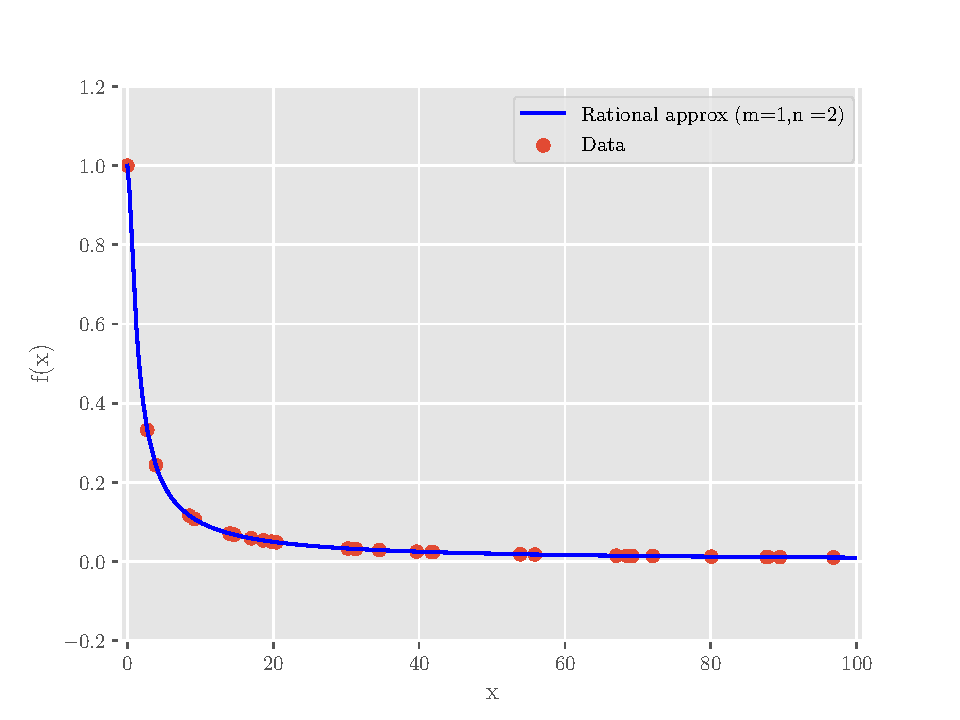
\includegraphics[width=.98\textwidth]{code/test04_01_2.pdf}
        \end{center}
    \end{minipage}%
    \begin{minipage}{.04\textwidth}%
    \end{minipage}%
    \begin{minipage}{.48\textwidth}%
        \begin{center}
            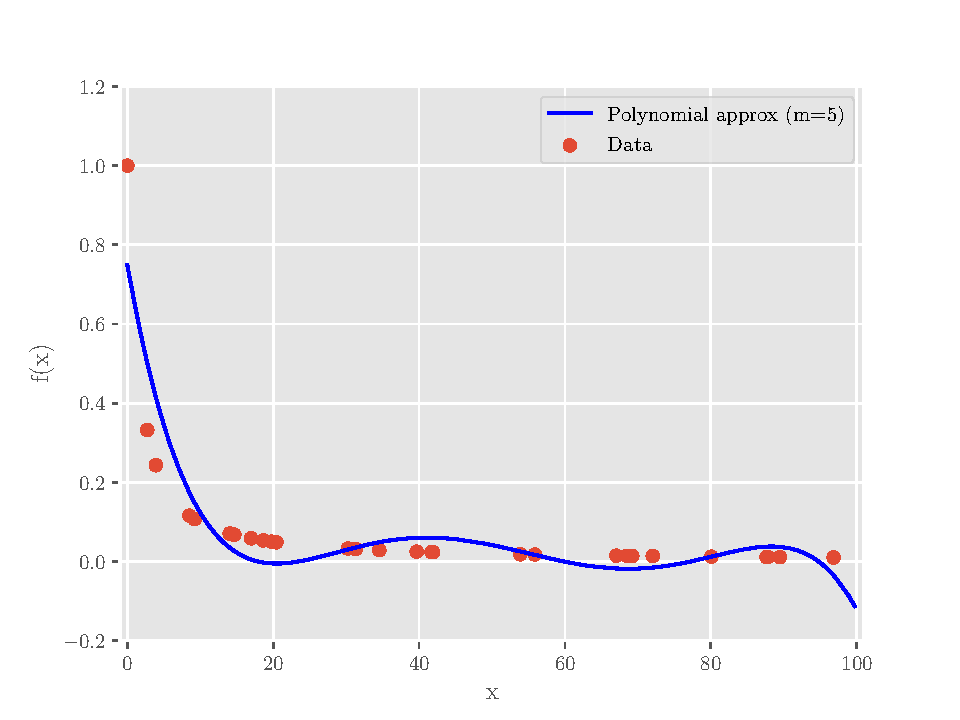
\includegraphics[width=.98\textwidth]{code/test04_05_0.pdf}
        \end{center}
    \end{minipage}%
    \centering
    \caption{Comparison of rational and polynomial approximation to input data
    that exhibits traits of a rational function. Left: rational approximation
with 6 coefficients. Right: polynomial approximation with 6 coefficients.}
    \label{fig:cmp}
\end{figure}





